\documentclass{article}
\usepackage[utf8]{inputenc}
\usepackage{subfig}
\usepackage{hyperref}
%References
\usepackage{natbib}
%IMPORTANT use https://www.citationmachine.net/ if you need to generate references!
% \citep{reference} creates Harvard Style references throughout

%Colors
\usepackage{xcolor}

\usepackage[protrusion=true,expansion]{microtype}

%Code Markup
\usepackage[outputdir=cache]{minted}
%Syntax Highlighting Style
\definecolor{bggray}{RGB}{40,40,40}
%Macro to make a Syntax Highlighter For Java files 
%Use \javacode{filename.java} to insert a Java File W/ Syntax Highlighting file into the PDF
\newmintedfile[javacode]{java}{
	style=fruity,
	bgcolor=bggray,
	linenos,
	breaklines,
	tabsize=2,
	obeytabs
}

\newmintedfile[bashoutput]{txt}{
	style=fruity,
	bgcolor=lightgray,
	breaklines,
	tabsize=2,
	obeytabs
}

%Page Margins and stuff
\usepackage{geometry}
 \geometry{
 a4paper,
 total={170mm,257mm},
 left=20mm,
 }

%Pictures
\usepackage{graphicx}
\graphicspath{ {./images/} }

%Move the title position
\usepackage{titling}

\setlength{\droptitle}{-8.5em} %Up, near the top but not too high

%Section Heading formatting
\usepackage{titlesec}

\titleformat{\section}
  {\normalfont\Large\bfseries}{\thesection}{1em}{}[{\titlerule[0.8pt]}]

\title{Group Project - Human Computer Interraction}
\author{Group 35: Daniel Hannon (19484286) Emanuel Wiesniewski (19469752)}
\date{November 2021}

\begin{document}
	\maketitle
	\section{Overview}
	\textbf{How to design learning systems that are appealing, attractive, and engaging to learners of different ages, personalities, educational background, and cultures? }\\
	\\
	Making suitable learning systems to cater to students from different backgrounds, personalities etc. is a difficult task. Within this report, we hope to outline issues with education and address an issue that affects many students across the world. Then we will attempt to approach this issue present a solution, then we will conclude with an evaluation.
	\section{User Needs}
	It's no secret that students all around the world struggle with organization. Especially in third level as most learning is ``Self Directed'' wherein the Student themselves must structure the regimine that they need to follow and then execute it and consequently this can cause a great deal of stress as it can be seen as some kind of unscalable task for some people, Especially people with disabilites. A lot of people going into higher education come straight from secondary school and as a result they also need to do a significantly higher amount of self management in terms of preparing food, working part-time, and the many things associated with living independently. \citep{aeonaguinis}\\ \\
	In fact, Good time management has been associated with higher GPA among full time and part time students \citep{maccanntime}, So it can be said that there's adequate reason to believe that a means to improve someones time management would be a very good way to ensure that they can perform to the best of their academic ability. In order to see what people would require we created a miro board and wrote up some User personas covering a diverse base of people who are in education. Including but not limited to:
		\begin{itemize}
			\item Mature Students
			\item Postgraduate Students
			\item Students Fresh from secondary school
			\item Students from different fields
			\item Leaving Certificate Students
			\item Students that may not be good with technology
		\end{itemize}\newpage
		Here is the Miro Board:
		\begin{figure}[h!]
			\begin{minipage}{0.5\linewidth}
				\centering
				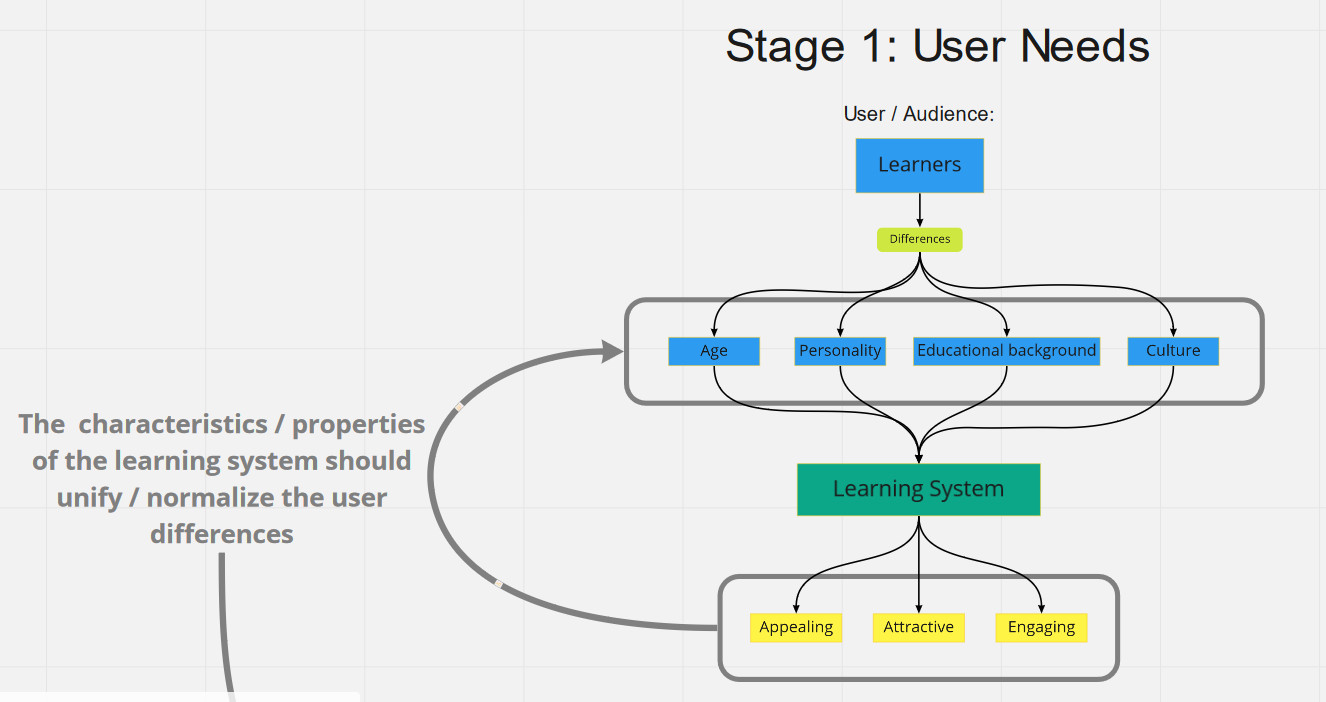
\includegraphics[width=0.9\textwidth]{userneeds.jpg}
				\caption{Step 1 (1/2)}
			\end{minipage}%
			\begin{minipage}{0.5\linewidth}
				\centering
				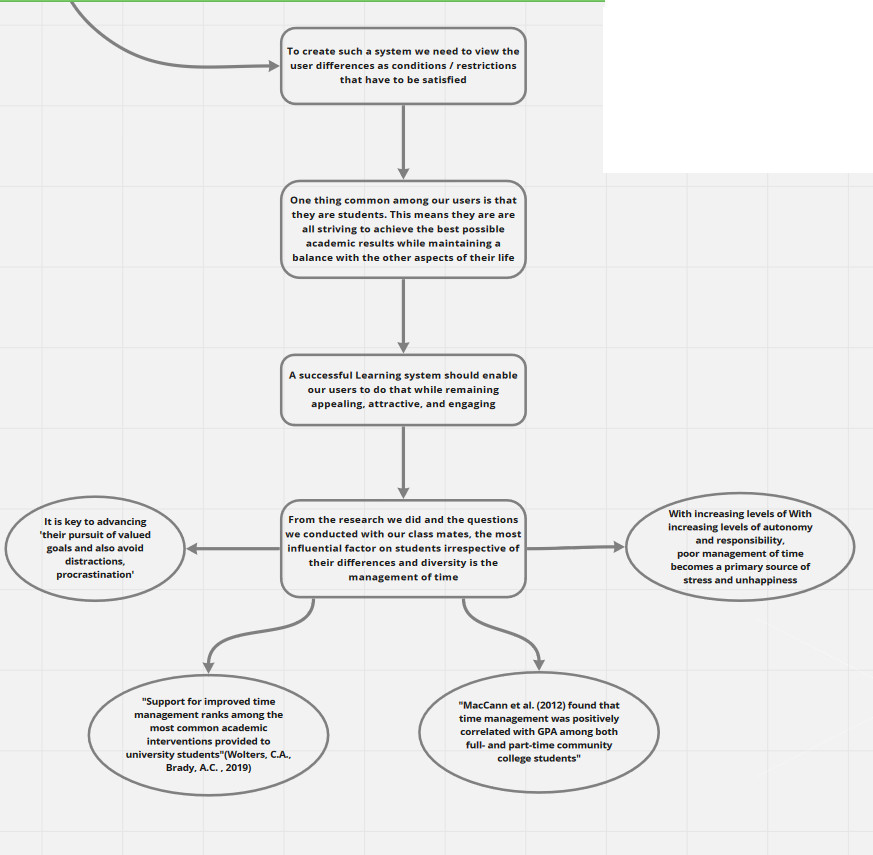
\includegraphics[width=0.9\textwidth]{userneeds2.jpg}
				\caption{Step 2 (2/2)}
			\end{minipage}
		\end{figure}
		\begin{figure}[h!]
			\centering
			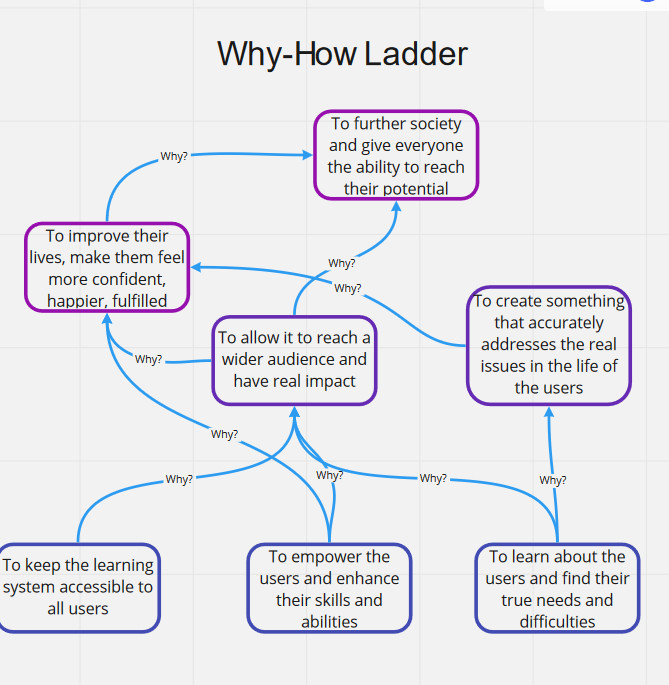
\includegraphics[width=0.7\textwidth]{whyhowladder.jpg}
		\end{figure}
		\newpage
		\begin{figure}[h!]
			\begin{minipage}{0.5\linewidth}
				\centering
				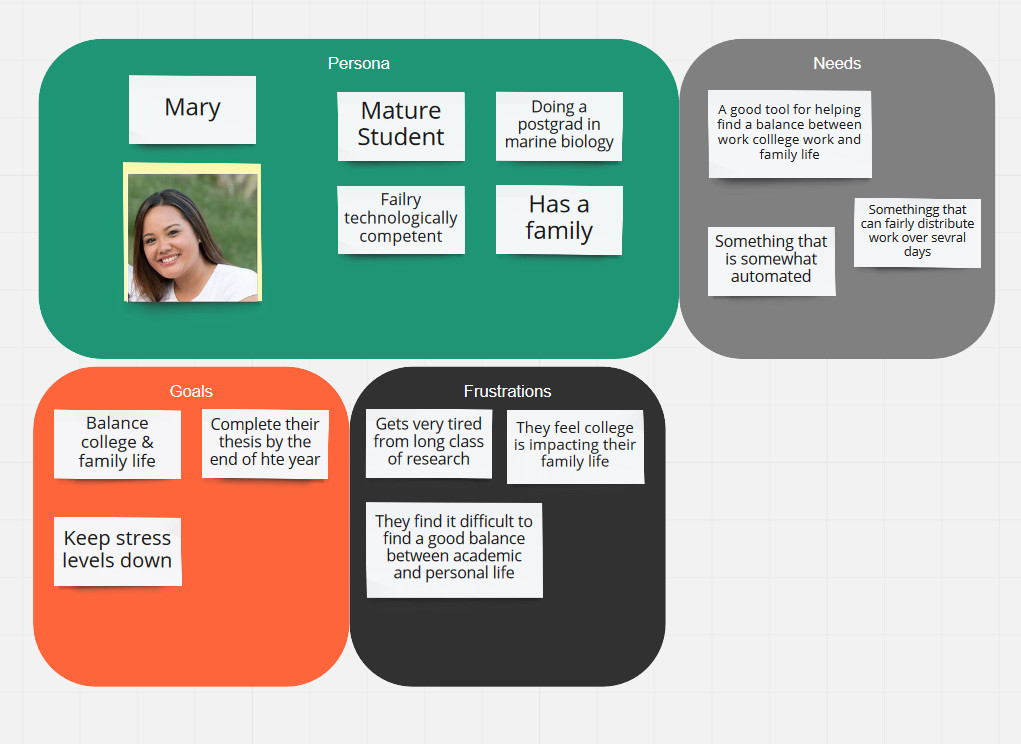
\includegraphics[width=0.9\textwidth]{userpersona1.jpg}
			\end{minipage}%
			\begin{minipage}{0.5\linewidth}
				\centering
				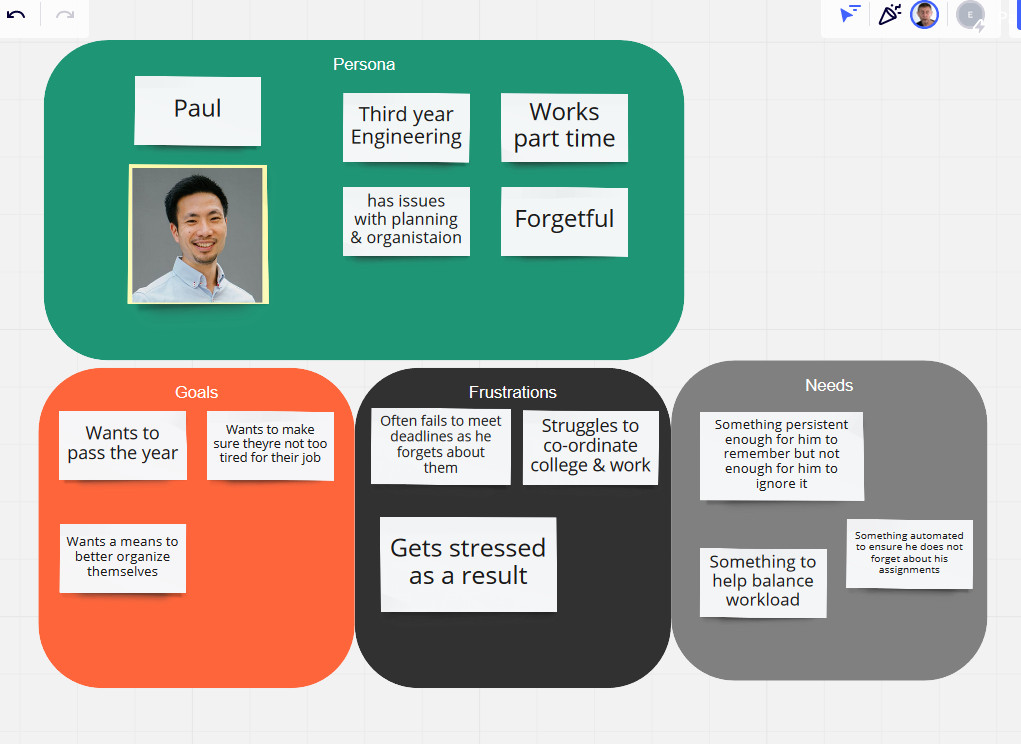
\includegraphics[width=0.9\textwidth]{userpersona2.jpg}
			\end{minipage}
		\end{figure}
		\begin{figure}[h!]
			\begin{minipage}{0.5\linewidth}
				\centering
				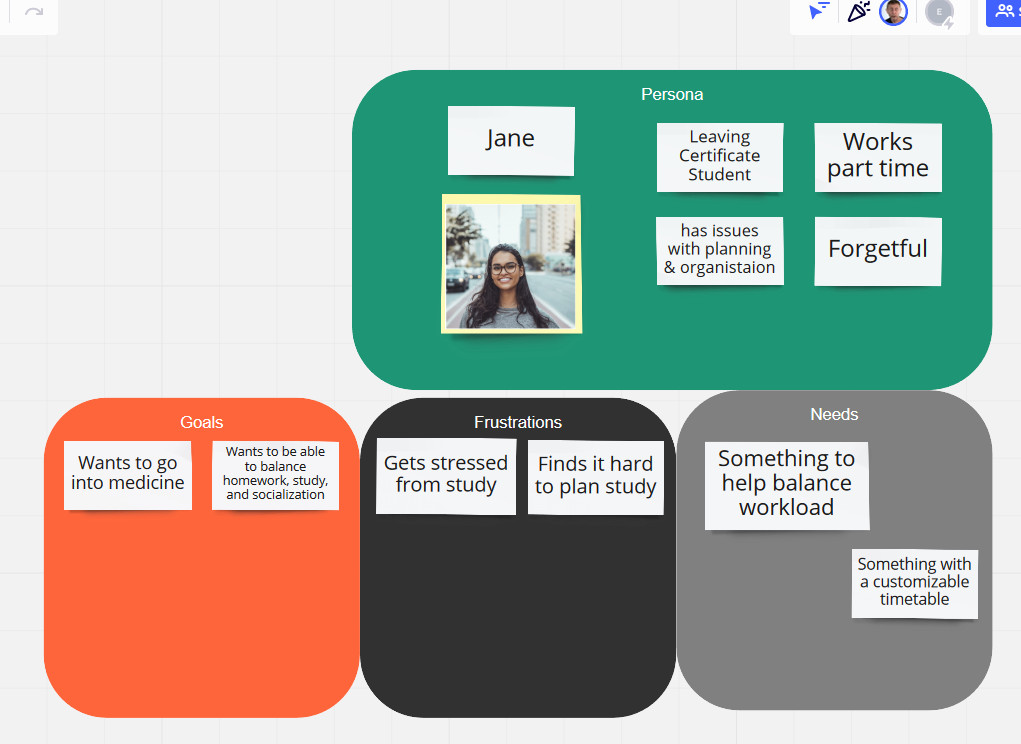
\includegraphics[width=0.9\textwidth]{userpersona3.jpg}
			\end{minipage}%
			\begin{minipage}{0.5\linewidth}
				\centering
				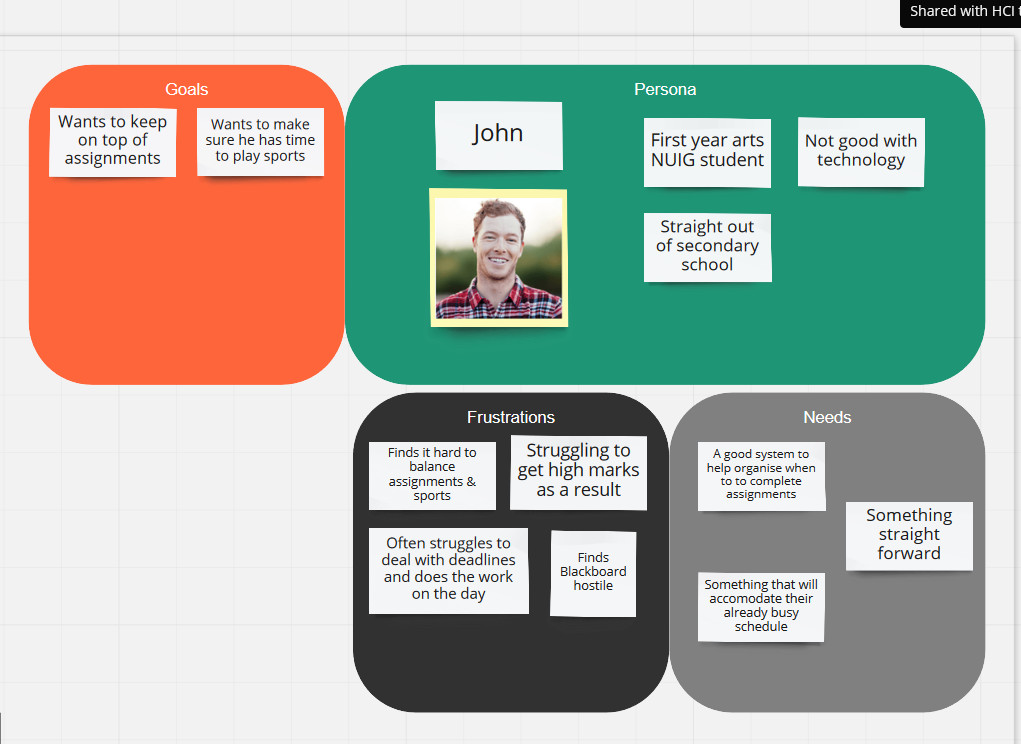
\includegraphics[width=0.9\textwidth]{userpersona4.jpg}
			\end{minipage}
		\end{figure}
		\begin{figure}[h!]
			\centering
			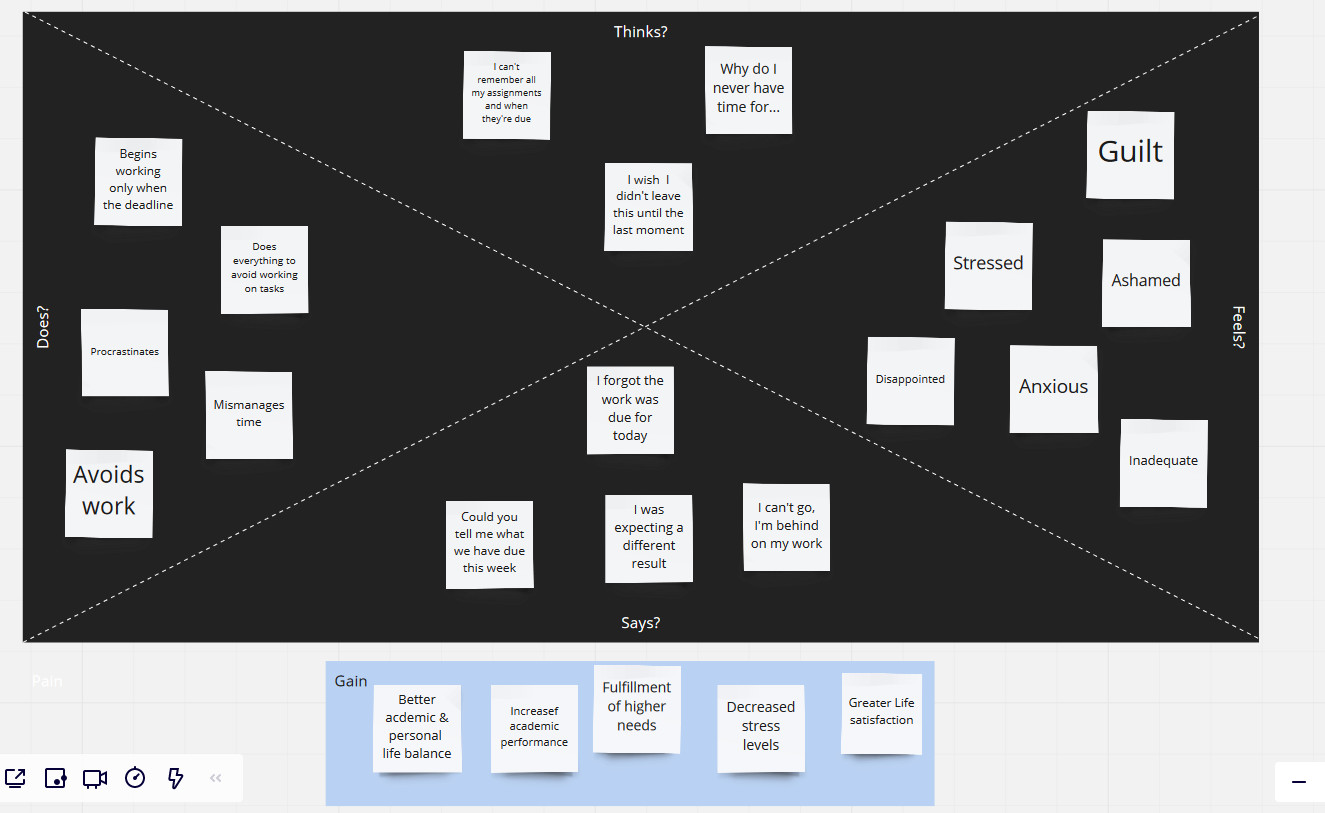
\includegraphics[width=0.8\textwidth]{empathymap.jpg}
		\end{figure}
	\newpage
		\begin{figure}[h!]
			\centering
			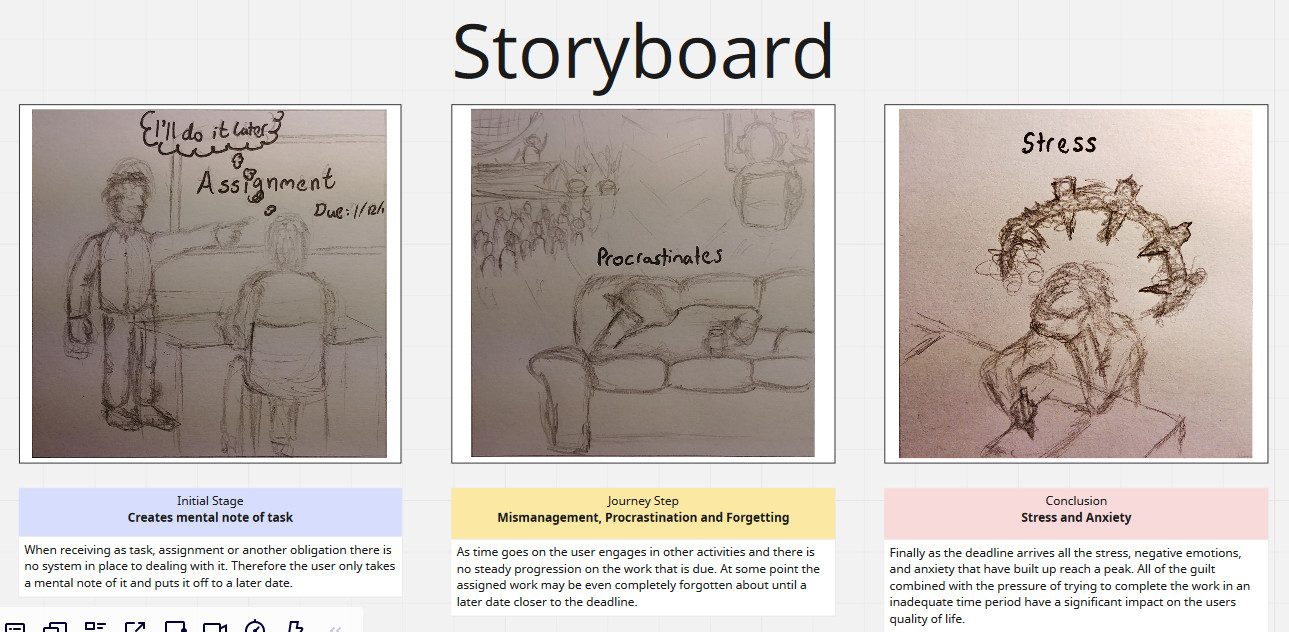
\includegraphics[width=0.8\textwidth]{storyboard1.jpg}
		\end{figure}
		\begin{figure}[h!]
			\centering
			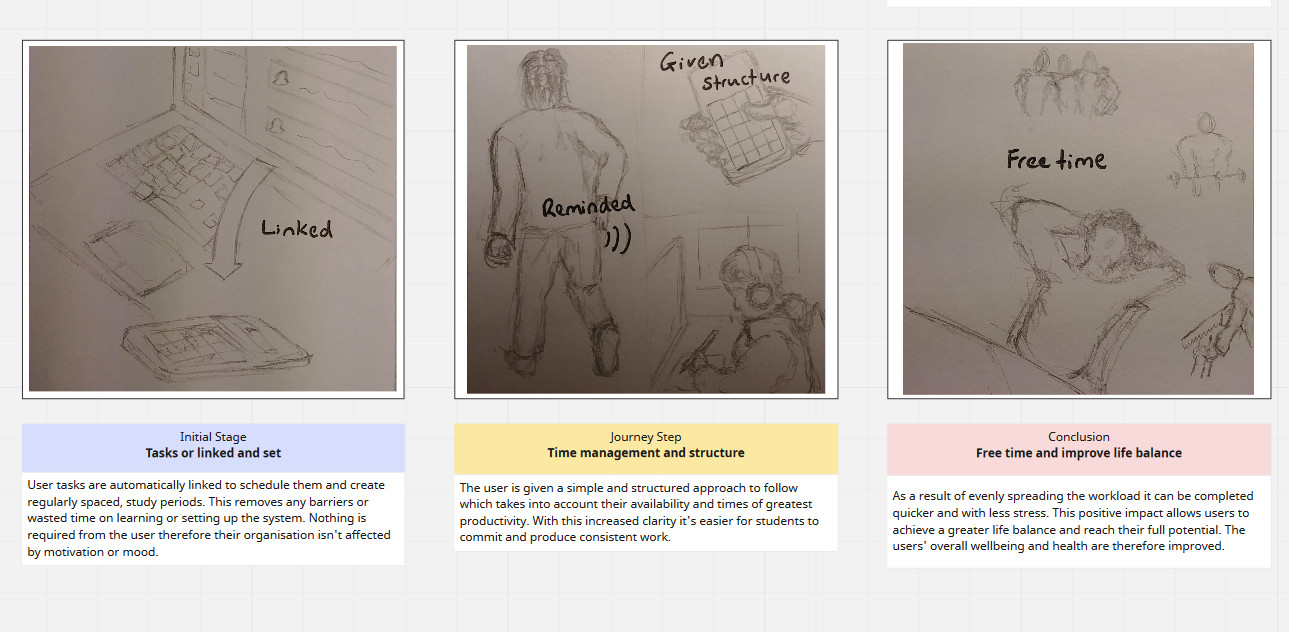
\includegraphics[width=0.8\textwidth]{storyboard2.jpg}
		\end{figure}
		\begin{figure}[h!]
			\centering
			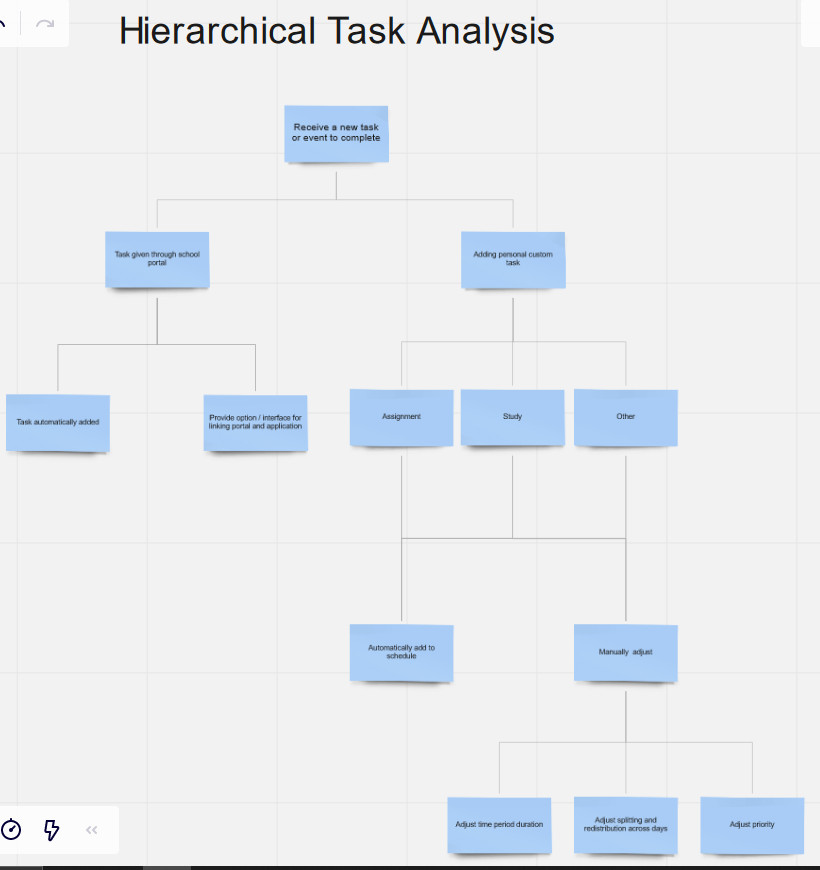
\includegraphics[width=0.5\textwidth]{hta.jpg}
		\end{figure}
		View in full size here: \href{https://miro.com/app/board/o9J_ljlqUA4=/?invite_link_id=328659315881}{https://miro.com/app/board/o9J\_ljlqUA4=/?invite\_link\_id=328659315881}
	\newpage
	\section{Interactive Prototype}
	In order to create the prototype we decided upon the software Figma as it made it very easy to create an interactive prototype. We decided upon creating a phone application as most people have smartphones. From what we established from the User Needs Evaluation we know the software needs to be. We Tried to adhere as much as possible to Dieter Rams 10 principles of design which are:
	\begin{itemize}
		\item \textbf{Innovative} - The Software must solve a given problem in a practical and effective way
		\item \textbf{Useful} - It must serve some kind of practical purpose
		\item \textbf{Aesthetic} - It must look good
		\item \textbf{Understandable} - There should be as little abstraction between each setting and menu and what they effect.
		\item \textbf{Unobtrusive} - It must not interfere with what the User needs in a negative way
		\item \textbf{Honest} - It should not lie about what it does, WYSIWYG (What You See Is What You Get) 
		\item \textbf{Long-Lasting} - It should not follow a trend as trends come and go
		\item \textbf{Thorough down to the last detail} - Every aspect of the  software must be designed
		\item \textbf{Environmentally Friendly} - In terms of software, rather than hardware it must accommodate the device in a means which does not make it User Hostile (Make every screen simple)
		\item \textbf{As little Design as possible} - It must not be over-engineered or have lots of distractions to pull you away from the problem it aims to solve.
	\end{itemize}  
	In order to adhere to this we decided to not overwhelm the user with distracting colors or anything like that. We also made buttons descriptive enough that the user immediately knows what they do, but not so descriptive that they are lost in what text is present. We designed this as a paper prototype:
	\begin{figure}[h!]
		\centering
		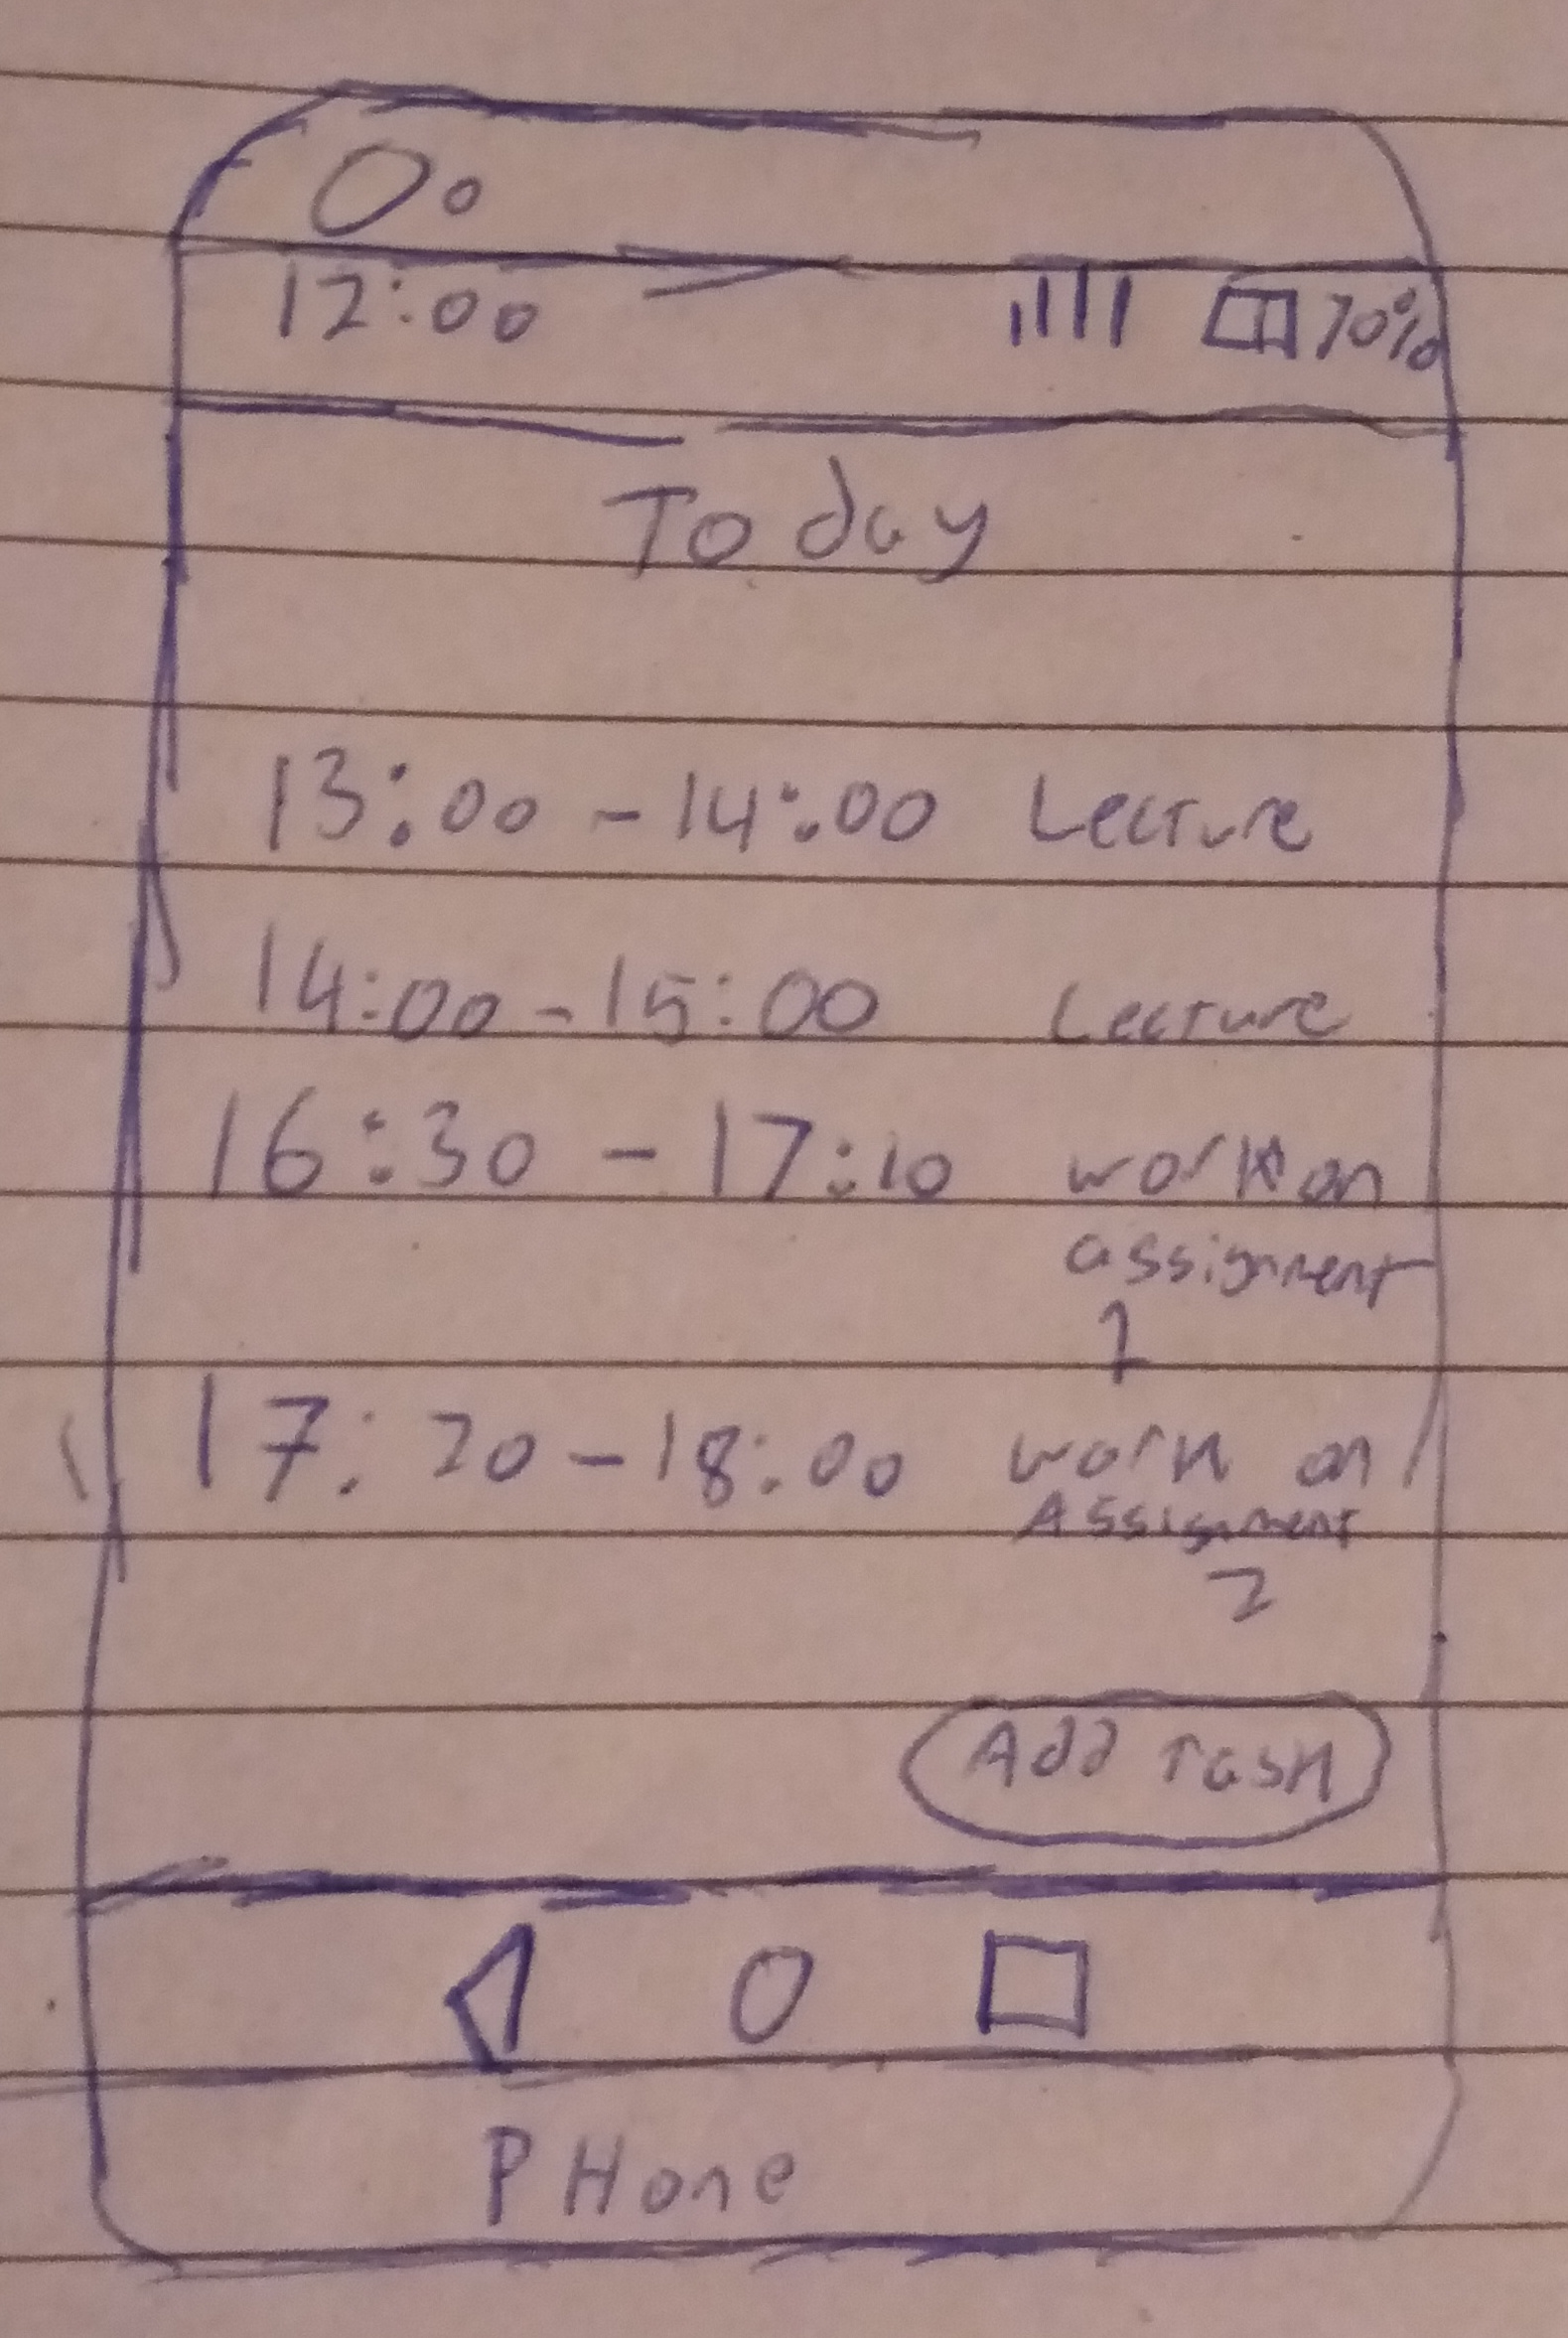
\includegraphics[width=0.5\textwidth]{1.jpg}
	\end{figure}\\
	In regards to features for the prototype, from the user needs stage we felt that something which helps students divide up time would help a lot, and something that could automatically pull what assignments are due from blackboard (or a similar platform) would help even more. As no two students are the same we figured that they would also need the ability to set the boundaries in which they are able to work between, and the amount of time they feel they can work without breaks (The Pomodoro Technique uses 25 minute bursts with 5-10 minute breaks for example) adn then allocate break times. Additionally we need to consider students who may not be enrolled in a university with an online hub to recieve their assignment data so we need a means to create tasks for them too. Additionally we want to create something to accomodate for non-assignment tasks such as study sessions.\\
		\begin{figure}[h!]
			\centering
			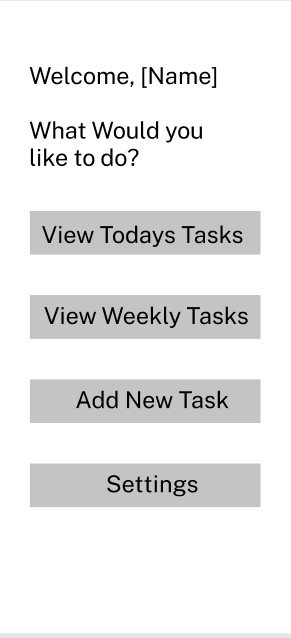
\includegraphics[width=0.25\textwidth]{menu.jpg}
		\end{figure}\\
	We decided upon this for the menu as we felt it would be as straightforward as possible. Each Button says exactly what it does, and the application greets you with your name to add some degree of human touch to the entire thing. \newpage
	\begin{figure}[h!]
		\centering
		\begin{minipage}{0.5\textwidth}
			\centering
			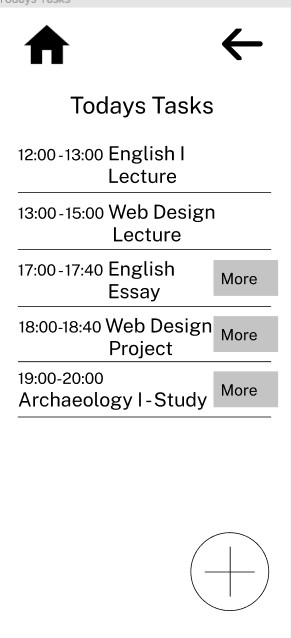
\includegraphics[width=0.5\textwidth]{todaystasks.jpg}
			\caption{Todays Tasks Viewer}
		\end{minipage}%
		\begin{minipage}{0.5\textwidth}
			\centering
			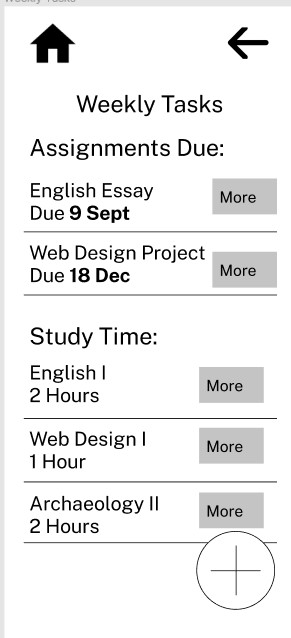
\includegraphics[width=0.5\textwidth]{weeklytasks.jpg}
			\caption{Weekly Tasks Viewer}
		\end{minipage}
	\end{figure} 
	Today and this weeks task menus show the same data but in a different way. Todays Tasks assigns times in which you can work on the assignments and study where Weekly Tasks says when your assignments are due and how long you will spend on studying if you adhere to the timetable that the application provides you.\\
	\begin{figure}[h!]
		\centering
		\begin{minipage}{0.5\textwidth}
			\centering
			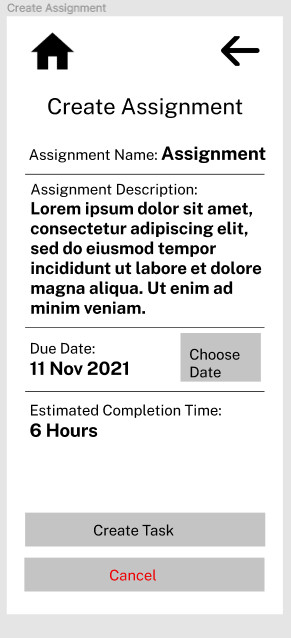
\includegraphics[width=0.5\textwidth]{createassignment.jpg}
			\caption{Assignment Creator interface}
		\end{minipage}%
		\begin{minipage}{0.5\textwidth}
			\centering
			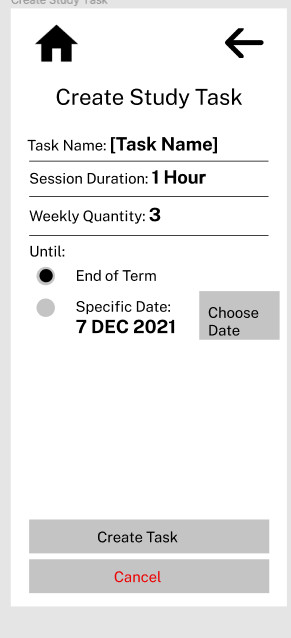
\includegraphics[width=0.5\textwidth]{createstudy.jpg}
			\caption{Create Study Task Interface}
		\end{minipage}
	\end{figure} 
	\\Assignment Creator and Study Task interfaces are very self explanatory and allow for customization such as allocating an estimated compketion time so the app makes sure to allocate appropriate quantities of time to work on the assignments given. The Study task interface allows you to set study duration periods, the amount of times during a week, and until a certain date in case you need someextra prep before a class test or something. \\
	A more detailed demonstration of the interactive prototype can be found here: \href{https://youtu.be/DZVVTVaetJ8}{https://youtu.be/DZVVTVaetJ8}\\
	The interactive demo for the prototype can be found here:\\ \href{https://www.figma.com/file/uc4K5MlmnyjnSnxDE55tnE/Prototype?node-id=0%3A1}{https://www.figma.com/file/uc4K5MlmnyjnSnxDE55tnE/Prototype?node-id=0\%3A1}
	
	\section{Evaluation}
	%Sets to Harvard Style and links the references file
	\subsection{Evaluation Based on User Experience}
	\begin{itemize}
		\item \textbf{Useful} - The purpose the product provides - help students with a key aspect of learning. It is designed to simplify and organise the academic aspect of the user’s life to eliminate a major source of anxiety and create more free time that users can then allocate to other important aspects of their life.
		\item \textbf{Usable} - For the usability of our learning system, we had to agree on the minimum number of key features and functionality necessary for our system to perform its desired purpose. The diversity found across different ages, personalities, educational background, and cultures acted as a restriction, leading us to making our user interface as simple and accessible as possible. We were conflicted on the trade-off between creating a personalised tailored aesthetic and a simple minimal design but after multiple considerations of both approaches and the purpose for which our system was constructed, we decided on the latter.
		\item \textbf{Findable} -Our system being findable was another consideration for us when choosing the medium in which to implement our design. By making our platform digital and accessible on mobile device, operating systems we hoped it would give our application the greatest chances of being findable and providing potential for creating greater awareness by advertising. This still does not guarantee anything and in todays landscape, with so many other great offerings, preventing your product from becoming invisible in the crowd is arguably one of the most challenging aspects, with only having the ability to influence the chances discoverability.
		\item \textbf{Credible} - Seeing that we aren’t creating a real product but only reaching the prototyping stage this aspect isn’t as applicable as the others. Brands pool resources and years of work into creating an image and reputation which users can trust. However, the intentions and motivations behind a product in our opinion are also important to consider and with our prototype we focused on fulfilling our users’ needs and kept this consideration in mind throughout the process.
		\item \textbf{Desirable} - As discussed in the usability section, the restrictions implied by user diversity and the design decisions we made because of this, unfortunately did limit, and impact the desirability aspect of our prototype. We found that the aesthetic aspect was the only concern expressed by users testing our prototype but also discovered that the primary source of desirability for our product originated from its functionality, simplicity and accessibility which were our priorities when developing it.
		\item \textbf{Accessible} - As outlined in the usability stage, we designed the system with simplicity in mind, however we had to choose some platform or medium to develop our system on. We decided that today mobile computing systems such as phones or wearable tech provided us with a good balance of being both portable (allows access from anywhere) and powerful enough to provide the features we concluded to be necessary to provide the key functionality. This solution naturally has many limitations, with a minimalistic UI design we hoped to include as much of our target market as possible students – of different ages, personalities, educational background, and cultures. However, there are exceptions we didn’t account for such as students with certain types of impairments or disabilities or students who do not have access to systems on which our platform is available. Despite this we feel this was an appropriate route when we consider the prevalence of mobile technology users in todays world and the capabilities it already provides for certain demographics (voice operation).
		\item \textbf{Valuable} - Unique feature set when compared to other time management systems, automatic assignment, learns user behaviour – enormous time saving, simple interface and a manageable learning curve. Unlike other time management programs, users don’t need to spend their precious time learning the software and wasting their time assigning tasks. The learning system attempts to remove as many barriers as possible and tries to support student in an area that will produce a positive effect on their life
	\end{itemize}
	\subsection{Peer Review}
	We presented the application to some of our peers as a means of getting some form of feedback on the design, Overall they found it very intuitive and one of our peers said that ``\textit{if it were real, I'd[sic] be using it all the time}''. The sole point of contention was the very plain interface primarily the use of a white background, two of our peers suggested we replace it with a simple pastel color and it'd be more palatable, although they were not too keen on the choice of background color, they still said that it would be something they would use if it were real.
	\bibliographystyle{agsm}
	\bibliography{references}
\end{document}